\icode{N24-MM-CA-L3-261010-001}
\nceeID[14]{新课标\Rmnum{2}}{25}
如图，一长度\(l =\) \,\qty{1.0}{m}的均匀薄板初始时静止在一光滑平台上，薄板的右端与平台的边缘\(O\)对齐。薄板上的一小物块从薄板的左端以某一初速度向右滑动，当薄板运动的距离\(\Delta l = \frac{l}{6}\)时，物块从薄板右端水平飞出；当物块落到地面时，薄板中心恰好运动到\(O\)点。已知物块与薄板的质量相等。它们之间的动摩擦因数\(\mu = 0.3\)，重力加速度大小\(g =\) \,\qty{10}{m/s^2}。求
\begin{enumerate}
    \item 物块初速度大小及其在薄板上运动的时间；
    \item 平台距地面的高度。
\end{enumerate}

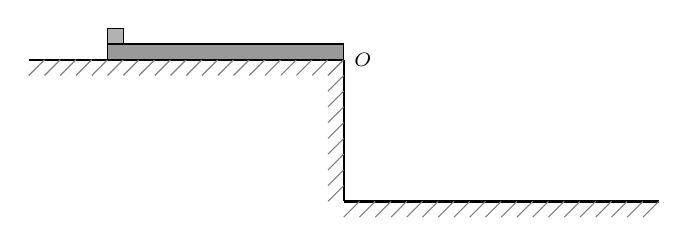
\begin{tikzpicture}[font=\scriptsize]
    \draw[thick] (-4,0)--(0,0)node[right]{\(O\)};
    \foreach \x in {-4,-3.8,...,-.2}
        \draw[gray] (\x,-.2)--++(.2,.2);
    \draw[thick] (0,0)--(0,-1.8);
    \foreach \y in {-1.8,-1.6,...,-.2}
        \draw[gray] (-.2,\y)--++(.2,.2);
    \draw[thick] (0,-1.8)--(4,-1.8);
    \foreach \x in {0,.2,...,3.8}
        \draw[gray] (\x,-2)--++(.2,.2);
    \draw[fill=gray!80] (-3,0) rectangle(0,.2);
    \draw[fill=gray!60] (-3,.2) rectangle(-2.8,.4);
 \end{tikzpicture}